% MORPH Architecture — Overview Diagram (vertical, labels horizontal)
% Compile: pdflatex morph_overview.tex

\documentclass[border=14pt]{standalone}
\usepackage[T1]{fontenc}
\usepackage{tikz}
\usetikzlibrary{
  arrows.meta, fit, positioning, calc,
  backgrounds, decorations.pathreplacing,
}

% ── Palette (colorblind-safe) ────────────────────────────────────────────────
\definecolor{cbBlue}{HTML}{4477AA}
\definecolor{cbOrange}{HTML}{EE7733}
\definecolor{cbPurple}{HTML}{AA3377}
\definecolor{cbTeal}{HTML}{228833}

\definecolor{fBlue}{HTML}{DCEAF7}
\definecolor{fOrange}{HTML}{FDE8D0}
\definecolor{fPurple}{HTML}{EEDCEE}
\definecolor{fTeal}{HTML}{D4EDDA}
\definecolor{fYellow}{HTML}{FFF3CD}
\definecolor{fGray}{HTML}{EBEBEB}

\definecolor{bdr}{HTML}{555555}
\definecolor{loopC}{HTML}{2255AA}
\definecolor{memC}{HTML}{AA3377}

\tikzset{
  B/.style={draw=bdr, thick, rounded corners=4pt,
    minimum width=5.0cm, minimum height=0.9cm,
    font=\small\sffamily, align=center, inner sep=5pt},
  Bs/.style={B, minimum height=0.55cm, font=\footnotesize\sffamily},
  Bm/.style={draw=memC, thick, rounded corners=4pt,
    minimum width=3.2cm, minimum height=0.7cm,
    font=\footnotesize\sffamily, align=center,
    fill=fPurple!70, inner sep=4pt},
  Bt/.style={draw=bdr, rounded corners=3pt,
    minimum width=3.2cm, minimum height=0.6cm,
    font=\footnotesize\sffamily, align=center, inner sep=3pt},
  A/.style={-{Stealth[length=2.5mm,width=2mm]}, thick},
  Ad/.style={-{Stealth[length=2.2mm,width=1.8mm]}, thick, densely dashed},
  ph/.style={font=\small\sffamily\bfseries},
  sub/.style={font=\scriptsize\sffamily},
}

\begin{document}
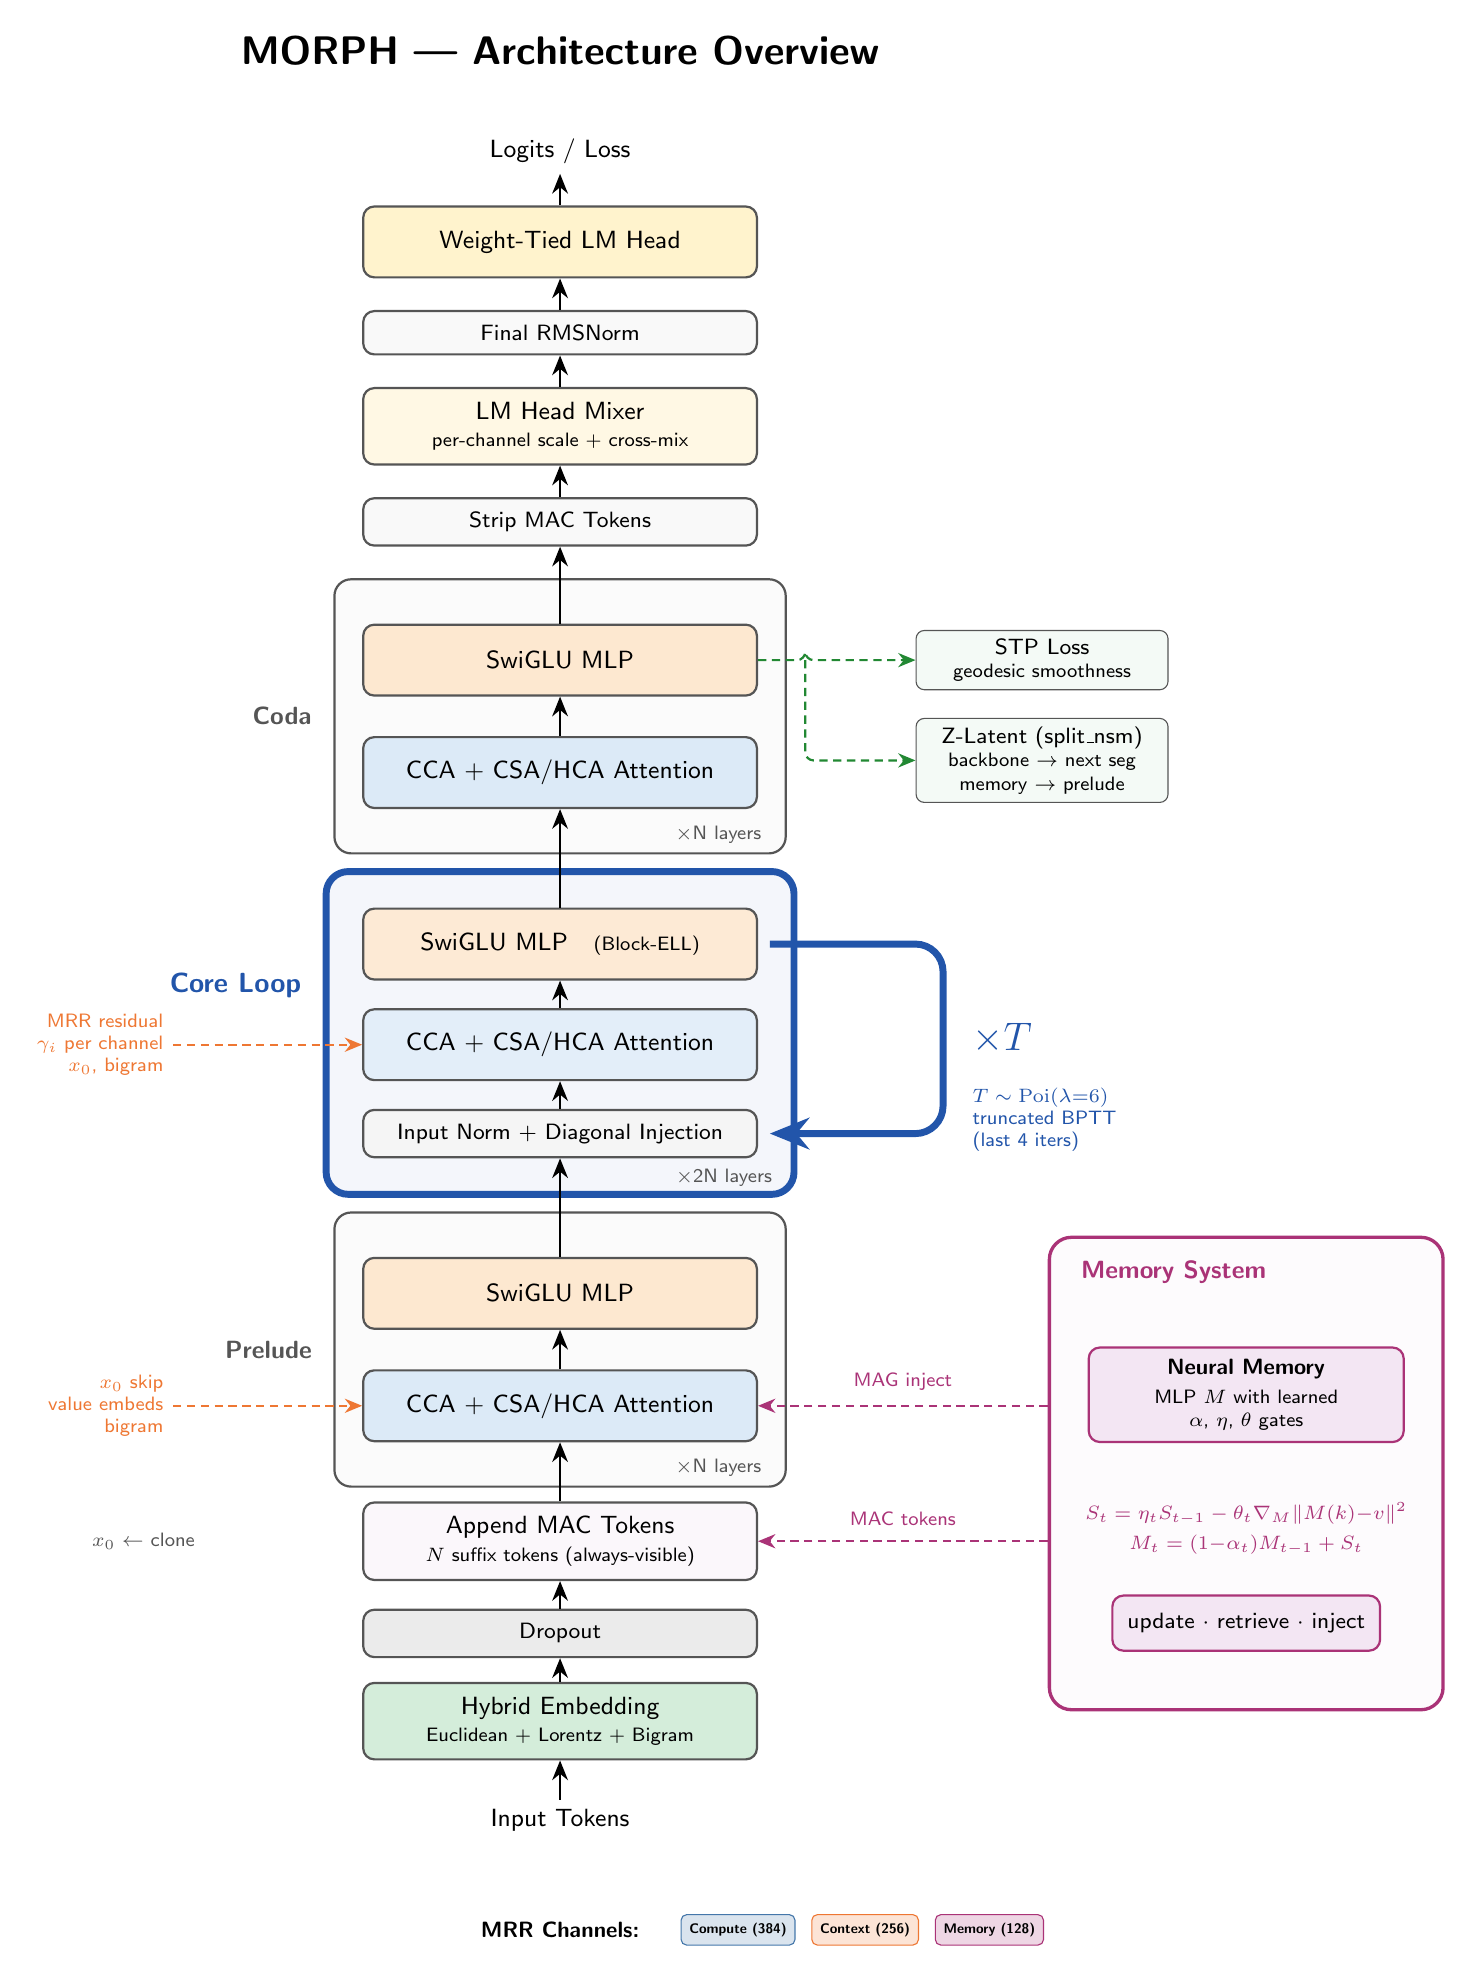
\begin{tikzpicture}[node distance=0.50cm]

% =====================================================================
% MAIN COLUMN
% =====================================================================

\node[font=\small\sffamily] (inp) {Input Tokens};

\node[B, fill=fTeal, above=0.5cm of inp] (emb) {
  Hybrid Embedding\\[-1pt]{\scriptsize Euclidean + Lorentz + Bigram}};
\draw[A] (inp) -- (emb);

\node[Bs, fill=fGray, above=0.3cm of emb] (drp) {Dropout};
\draw[A] (emb) -- (drp);

% ── MAC TOKENS (right after embedding, before any layers) ────────────
\node[B, fill=fPurple!22, above=0.35cm of drp] (mac) {
  Append MAC Tokens\\[-1pt]{\scriptsize $N$ suffix tokens (always-visible)}};
\draw[A] (drp) -- (mac);

\node[sub, text=bdr, left=2.0cm of mac] {$x_0 \leftarrow$ clone};

% ── PRELUDE ──────────────────────────────────────────────────────────
\node[B, fill=fBlue, above=0.75cm of mac] (pa) {CCA + CSA/HCA Attention};
\node[B, fill=fOrange, above=0.5cm of pa] (pm) {SwiGLU MLP};
\draw[A] (mac) -- (pa);
\draw[A] (pa) -- (pm);

\begin{scope}[on background layer]
  \node[draw=bdr, thick, rounded corners=6pt, fill=fGray!20,
        fit=(pa)(pm), inner xsep=10pt, inner ysep=16pt] (PG) {};
\end{scope}
\node[ph, anchor=east, text=bdr] at ($(PG.west)+(-0.15,0)$) {Prelude};
\node[sub, text=bdr, anchor=east] at ($(PG.south east)+(-0.2,0.25)$)
  {$\times$N layers};

\node[sub, text=cbOrange, left=2.4cm of pa, align=right]
  (psid) {$x_0$ skip\\value embeds\\bigram};
\draw[Ad, cbOrange] (psid.east) -- (pa.west);

% ── CORE LOOP ────────────────────────────────────────────────────────
\node[Bs, fill=fGray!50, above=1.25cm of pm] (inj) {
  Input Norm + Diagonal Injection};
\draw[A] (pm) -- (inj);

\node[B, fill=fBlue!80, above=0.35cm of inj] (ca) {CCA + CSA/HCA Attention};
\node[B, fill=fOrange!90, above=0.35cm of ca] (cm) {
  SwiGLU MLP\quad{\scriptsize (Block-ELL)}};
\draw[A] (inj) -- (ca);
\draw[A] (ca) -- (cm);

% Core loop box
\begin{scope}[on background layer]
  \node[draw=loopC, line width=2.5pt, rounded corners=8pt,
        fill=loopC!5, fit=(inj)(ca)(cm), inner sep=13pt] (CG) {};
\end{scope}
% Core Loop label — LEFT side, above the orange arrow line
\node[font=\normalsize\sffamily\bfseries, text=loopC, anchor=east]
  at ($(CG.west)+(-0.15,0.6)$) {Core Loop};
\node[sub, text=bdr, anchor=east] at ($(CG.south east)+(-0.2,0.25)$)
  {$\times$2N layers};
% Core side inputs
\node[sub, text=cbOrange, left=2.4cm of ca, align=right]
  (csid) {MRR residual\\$\gamma_i$ per channel\\$x_0$, bigram};
\draw[Ad, cbOrange] (csid.east) -- (ca.west);

% ── LOOP-BACK ARROW ─────────────────────────────────────────────────
\draw[loopC, line width=2.5pt, rounded corners=10pt,
      -{Stealth[length=5mm,width=4mm]}]
  ($(cm.east)+(0.15,0)$) -- ++(2.2,0) |- ($(inj.east)+(0.15,0)$);

% ×T label
\node[font=\Large\sffamily\bfseries, text=loopC, anchor=west]
  at ($(cm.east)+(2.6,-1.2)$) {$\times T$};

\node[sub, text=loopC, align=left, anchor=north west]
  at ($(cm.east)+(2.6,-1.7)$)
  {$T \sim \mathrm{Poi}(\lambda{=}6)$\\truncated BPTT\\(last 4 iters)};

% ── CODA ────────────────────────────────────────────────────────────
\node[B, fill=fBlue, above=1.25cm of cm] (da) {CCA + CSA/HCA Attention};
\node[B, fill=fOrange, above=0.5cm of da] (dm) {SwiGLU MLP};
\draw[A] (cm) -- (da);
\draw[A] (da) -- (dm);

\begin{scope}[on background layer]
  \node[draw=bdr, thick, rounded corners=6pt, fill=fGray!20,
        fit=(da)(dm), inner xsep=10pt, inner ysep=16pt] (DG) {};
\end{scope}
\node[ph, anchor=east, text=bdr] at ($(DG.west)+(-0.15,0)$) {Coda};
\node[sub, text=bdr, anchor=east] at ($(DG.south east)+(-0.2,0.25)$)
  {$\times$N layers};

% ── STRIP MAC + LM HEAD ────────────────────────────────────────────
\node[Bs, fill=fGray!30, above=0.4cm of DG] (str) {Strip MAC Tokens};
\draw[A] (dm) -- (str);

\node[B, fill=fYellow!55, above=0.4cm of str] (mix) {
  LM Head Mixer\\[-1pt]{\scriptsize per-channel scale + cross-mix}};
\draw[A] (str) -- (mix);

\node[Bs, fill=fGray!30, above=0.4cm of mix] (fn) {Final RMSNorm};
\draw[A] (mix) -- (fn);

\node[B, fill=fYellow, above=0.4cm of fn] (hd) {Weight-Tied LM Head};
\draw[A] (fn) -- (hd);

\node[font=\small\sffamily, above=0.4cm of hd] (out) {Logits / Loss};
\draw[A] (hd) -- (out);

% =====================================================================
% RIGHT: MEMORY SYSTEM
% =====================================================================

\coordinate (mem_anchor) at ($(mac.east)!0.5!(pa.east)+(6.2,0)$);

\node[draw=memC, very thick, rounded corners=8pt, fill=fPurple!10,
      minimum width=5.0cm, minimum height=6.0cm,
      inner sep=10pt, anchor=center] (MEM) at (mem_anchor) {};

\node[ph, text=cbPurple, anchor=north west]
  at ($(MEM.north west)+(0.3,-0.2)$) {Memory System};

\node[Bm, minimum width=4.0cm, minimum height=1.2cm]
  at ($(MEM.center)+(0,1.0)$) (mlp) {
  \textbf{Neural Memory}\\[1pt]
  {\scriptsize MLP $M$ with learned}\\[-1pt]
  {\scriptsize $\alpha$, $\eta$, $\theta$ gates}};

\node[sub, text=cbPurple, align=center] at ($(MEM.center)+(0,-0.7)$) {
  $S_t = \eta_t S_{t{-}1} - \theta_t \nabla_M \|M(k){-}v\|^2$\\[3pt]
  $M_t = (1{-}\alpha_t) M_{t{-}1} + S_t$};

\node[Bm, minimum width=3.4cm] at ($(MEM.center)+(0,-1.9)$) {
  update $\cdot$ retrieve $\cdot$ inject};

% ── Memory arrows (2 paths: MAG inject + MAC tokens) ────────────────

\draw[Ad, memC, rounded corners=4pt]
  (MEM.west |- pa) -- (pa.east)
  node[midway, above=2pt, sub, text=memC] {MAG inject};

\draw[Ad, memC, rounded corners=4pt]
  (MEM.west |- mac) -- (mac.east)
  node[midway, above=2pt, sub, text=memC] {MAC tokens};

% =====================================================================
% RIGHT: STP + Z-LATENT
% =====================================================================

\node[Bt, fill=fTeal!25, right=2.0cm of dm, minimum width=3.2cm] (stp) {
  STP Loss\\[-1pt]{\scriptsize geodesic smoothness}};

\node[Bt, fill=fTeal!25, below=0.35cm of stp, minimum width=3.2cm] (zlt) {
  Z-Latent (split\_nsm)\\[-1pt]
  {\scriptsize backbone $\to$ next seg}\\[-1pt]
  {\scriptsize memory $\to$ prelude}};

\coordinate (branch) at ($(dm.east)+(0.6,0)$);
\draw[Ad, cbTeal, rounded corners=3pt]
  (dm.east) -- (branch) |- (stp.west);
\draw[Ad, cbTeal, rounded corners=3pt]
  (branch) |- (zlt.west);

% =====================================================================
% LEGEND
% =====================================================================

\node[below=0.9cm of inp, font=\footnotesize\sffamily\bfseries] (leg)
  {MRR Channels:};
\node[right=0.4cm of leg, fill=cbBlue!20, draw=cbBlue,
      rounded corners=2pt, inner sep=3pt, font=\tiny\sffamily\bfseries]
  (l1) {Compute (384)};
\node[right=0.2cm of l1, fill=cbOrange!20, draw=cbOrange,
      rounded corners=2pt, inner sep=3pt, font=\tiny\sffamily\bfseries]
  (l2) {Context (256)};
\node[right=0.2cm of l2, fill=cbPurple!20, draw=cbPurple,
      rounded corners=2pt, inner sep=3pt, font=\tiny\sffamily\bfseries]
  (l3) {Memory (128)};

% ── Title ────────────────────────────────────────────────────────────
\node[above=0.7cm of out, font=\Large\sffamily\bfseries]
  {MORPH --- Architecture Overview};

\end{tikzpicture}
\end{document}
